%%%%%%%%%%%%%%%%%%%%%%%%%%%%%%%%%%%%%%%%%%%%%%%%%%%%%%%%%%%%%%%%%%%%%%%%
\clearpage
\section{Functions for analysing azimuthal averaged data}


%%%%%%%%%%%%%%%%%%%%%%%%%%%%%%%%%%%%%%%%%%%%%%%%%%%%%%%%%%%%%%%%%%%%%%%%%

%\clearpage
\subsection{$\sin^2$-$\sin^4$ azimuthal analysis} ~\\
This plugin can be used to describe azimuthal averaged data in case of e.g.\ magnetic scattering \cite{Wiedenmann2011}, where depending on the incident and scattered polarization and the dipole-dipole nature of the interaction of the neutron with a magnetic moment of an atom an angle dependent cross-section is observed even though the scattering objects are spherical. The spherical symmetry is broken by orienting the magnetic towards a applied magnetic field. Some detailed form factor for magnetic objects can be found in chapter \ref{sec:magneticstructures}. The scattering can be often decomposed in an isotropic term independent of the angle between the scattering vector and the applied field and anisotropic terms which anisotropy term is described by a $\sin^2(\psi)$ and $\sin^4(\psi)$ term.
\begin{align}
I_\mathrm{rad}(\psi) &= A + B\sin^2(\psi-\delta) + C \sin^4(\psi-\delta) \\
I_\mathrm{deg}(\psi) &= A + B\sin^2\left((\psi-\delta)\frac{\pi}{180}\right) + C \sin^4\left((\psi-\delta)\frac{\pi}{180}\right)
\end{align}

\hspace{1pt}\\
\underline{Input Parameters for models \texttt{A+Bsin2+Csin4 (deg)} and \texttt{A+Bsin2+Csin4 (rad)}:}\\
\begin{description}
\item[\texttt{A}] isotropic scattering intensity $A$
\item[\texttt{B}] anisotropic $\sin^2$-dependent scattering intensity $B$
\item[\texttt{C}] anisotropic $\sin^4$-dependent scattering intensity $C$
\item[\texttt{delta}] offset of deformation direction $\delta$ in degree or radian
\end{description}

\noindent \underline{Note:}
None.


\begin{figure}[htb]
\begin{center}
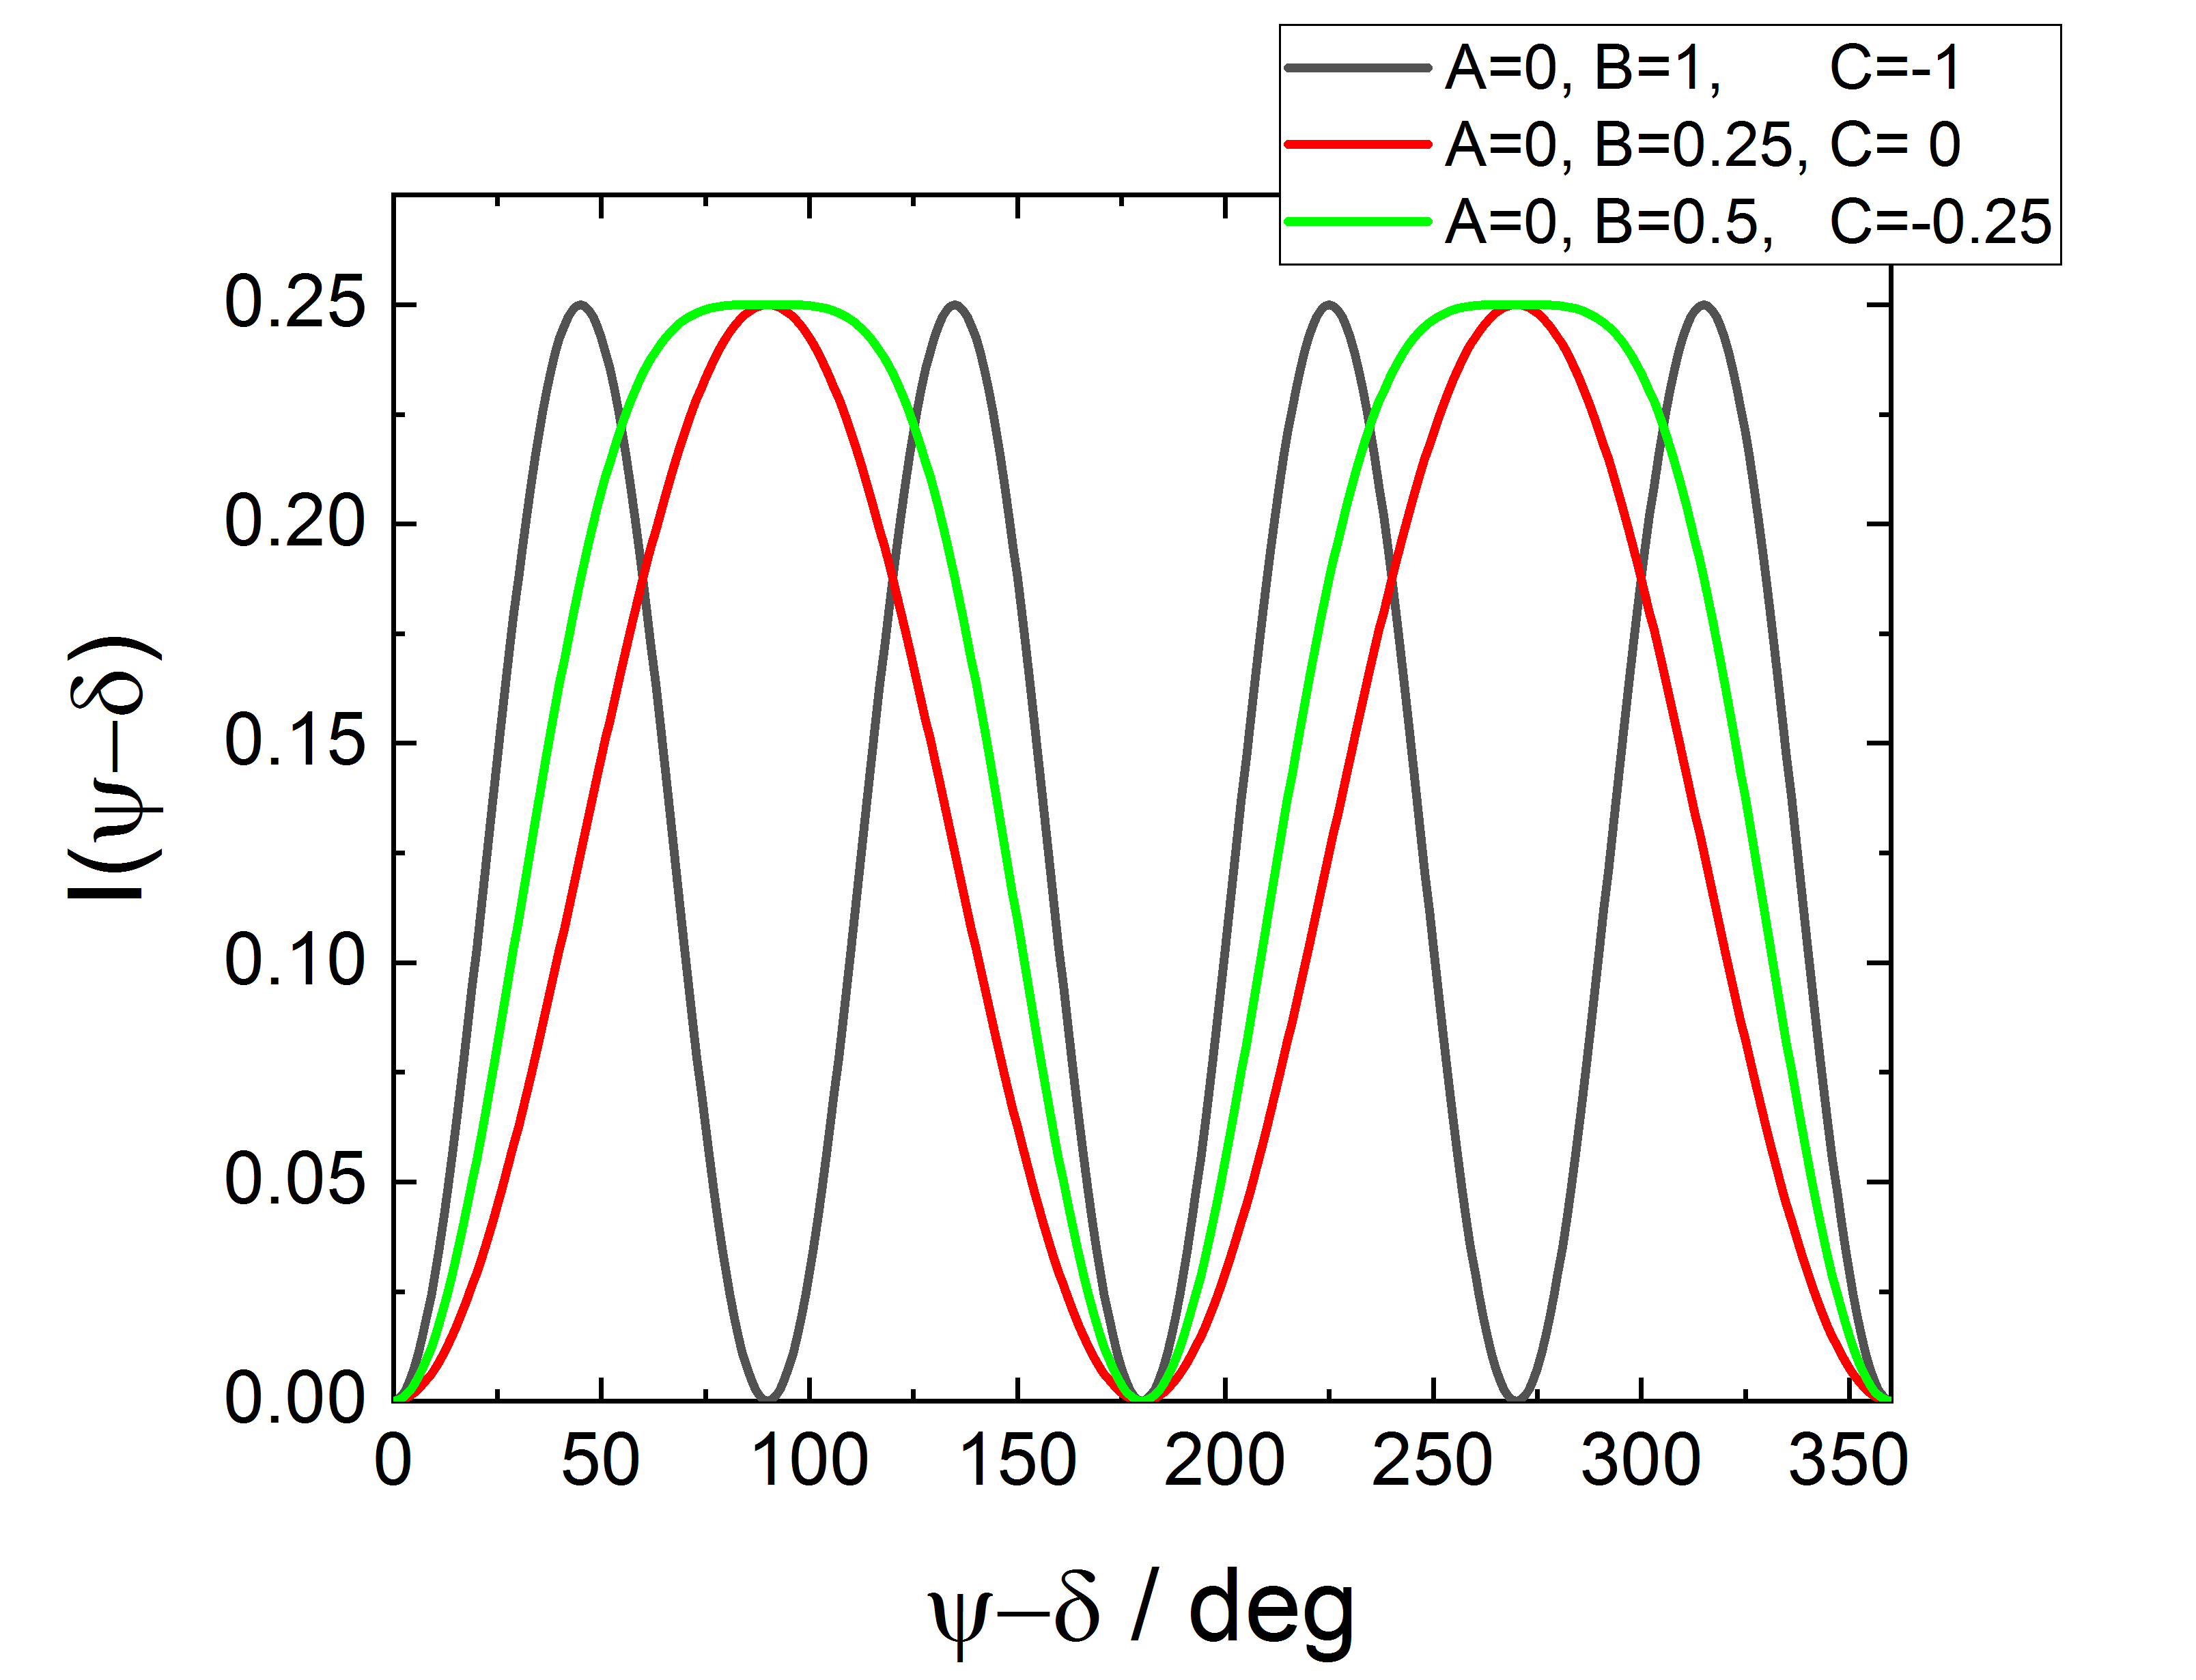
\includegraphics[width=0.7\textwidth]{../images/form_factor/azimuthal/sin2sin4.png}
\end{center}
\caption{Azimuthal intensity distribution typical in the field of magnetic scattering}
\label{fig:IQsin2sin4}
\end{figure}

\newpage
\subsection{Ellipsoidal azimuthal analysis} ~\\
Instead of radial or sector averaged data this function describes azimuthal averaged data of deformed or textured samples with an anisotropic scattering pattern as described in
\cite{Summerfield1983,Mildner1983,Reynolds1984,Hammouda1986,Hammouda1986a,Saraf1989,Svetogorsky1990,Gu2016,Gu2018}
\begin{align}
I_\mathrm{rad}(\psi) &= \left(\left(\frac{\cos(\psi-\delta)}{A}\right)^2 + \left(\frac{\sin(\psi-\delta)}{B}\right)^2\right)^{-N/2} +C\\
I_\mathrm{deg}(\psi) &= \left(\left(\frac{\cos\left((\psi-\delta)\frac{\pi}{180}\right)}{A}\right)^2 + \left(\frac{\sin\left((\psi-\delta)\frac{\pi}{180}\right)}{B}\right)^2\right)^{-N/2}+C
\end{align}
\hspace{1pt}\\
\underline{Input Parameters for models \texttt{elliptically averaged (deg)}} \underline{and} \underline{\texttt{elliptically averaged (rad)}:}\\
\begin{description}
\item[\texttt{A}] semi-axis along $\psi-\delta=0$ of iso-contours in reciprocal space
\item[\texttt{B}] semi-axis along $\psi-\delta=\pi/2$ of iso-contours in reciprocal space
\item[\texttt{C}] Amplitude $A$ of the angle dependent intensity
\item[\texttt{delta}] direction of the polarisation $\delta$ in degree or radian
\end{description}

\noindent \underline{Note:}
The reciprocal value of $A$ and $B$ are related to the corresponding correlation length of the scattering object in that direction.


\begin{figure}[htb]
\begin{center}
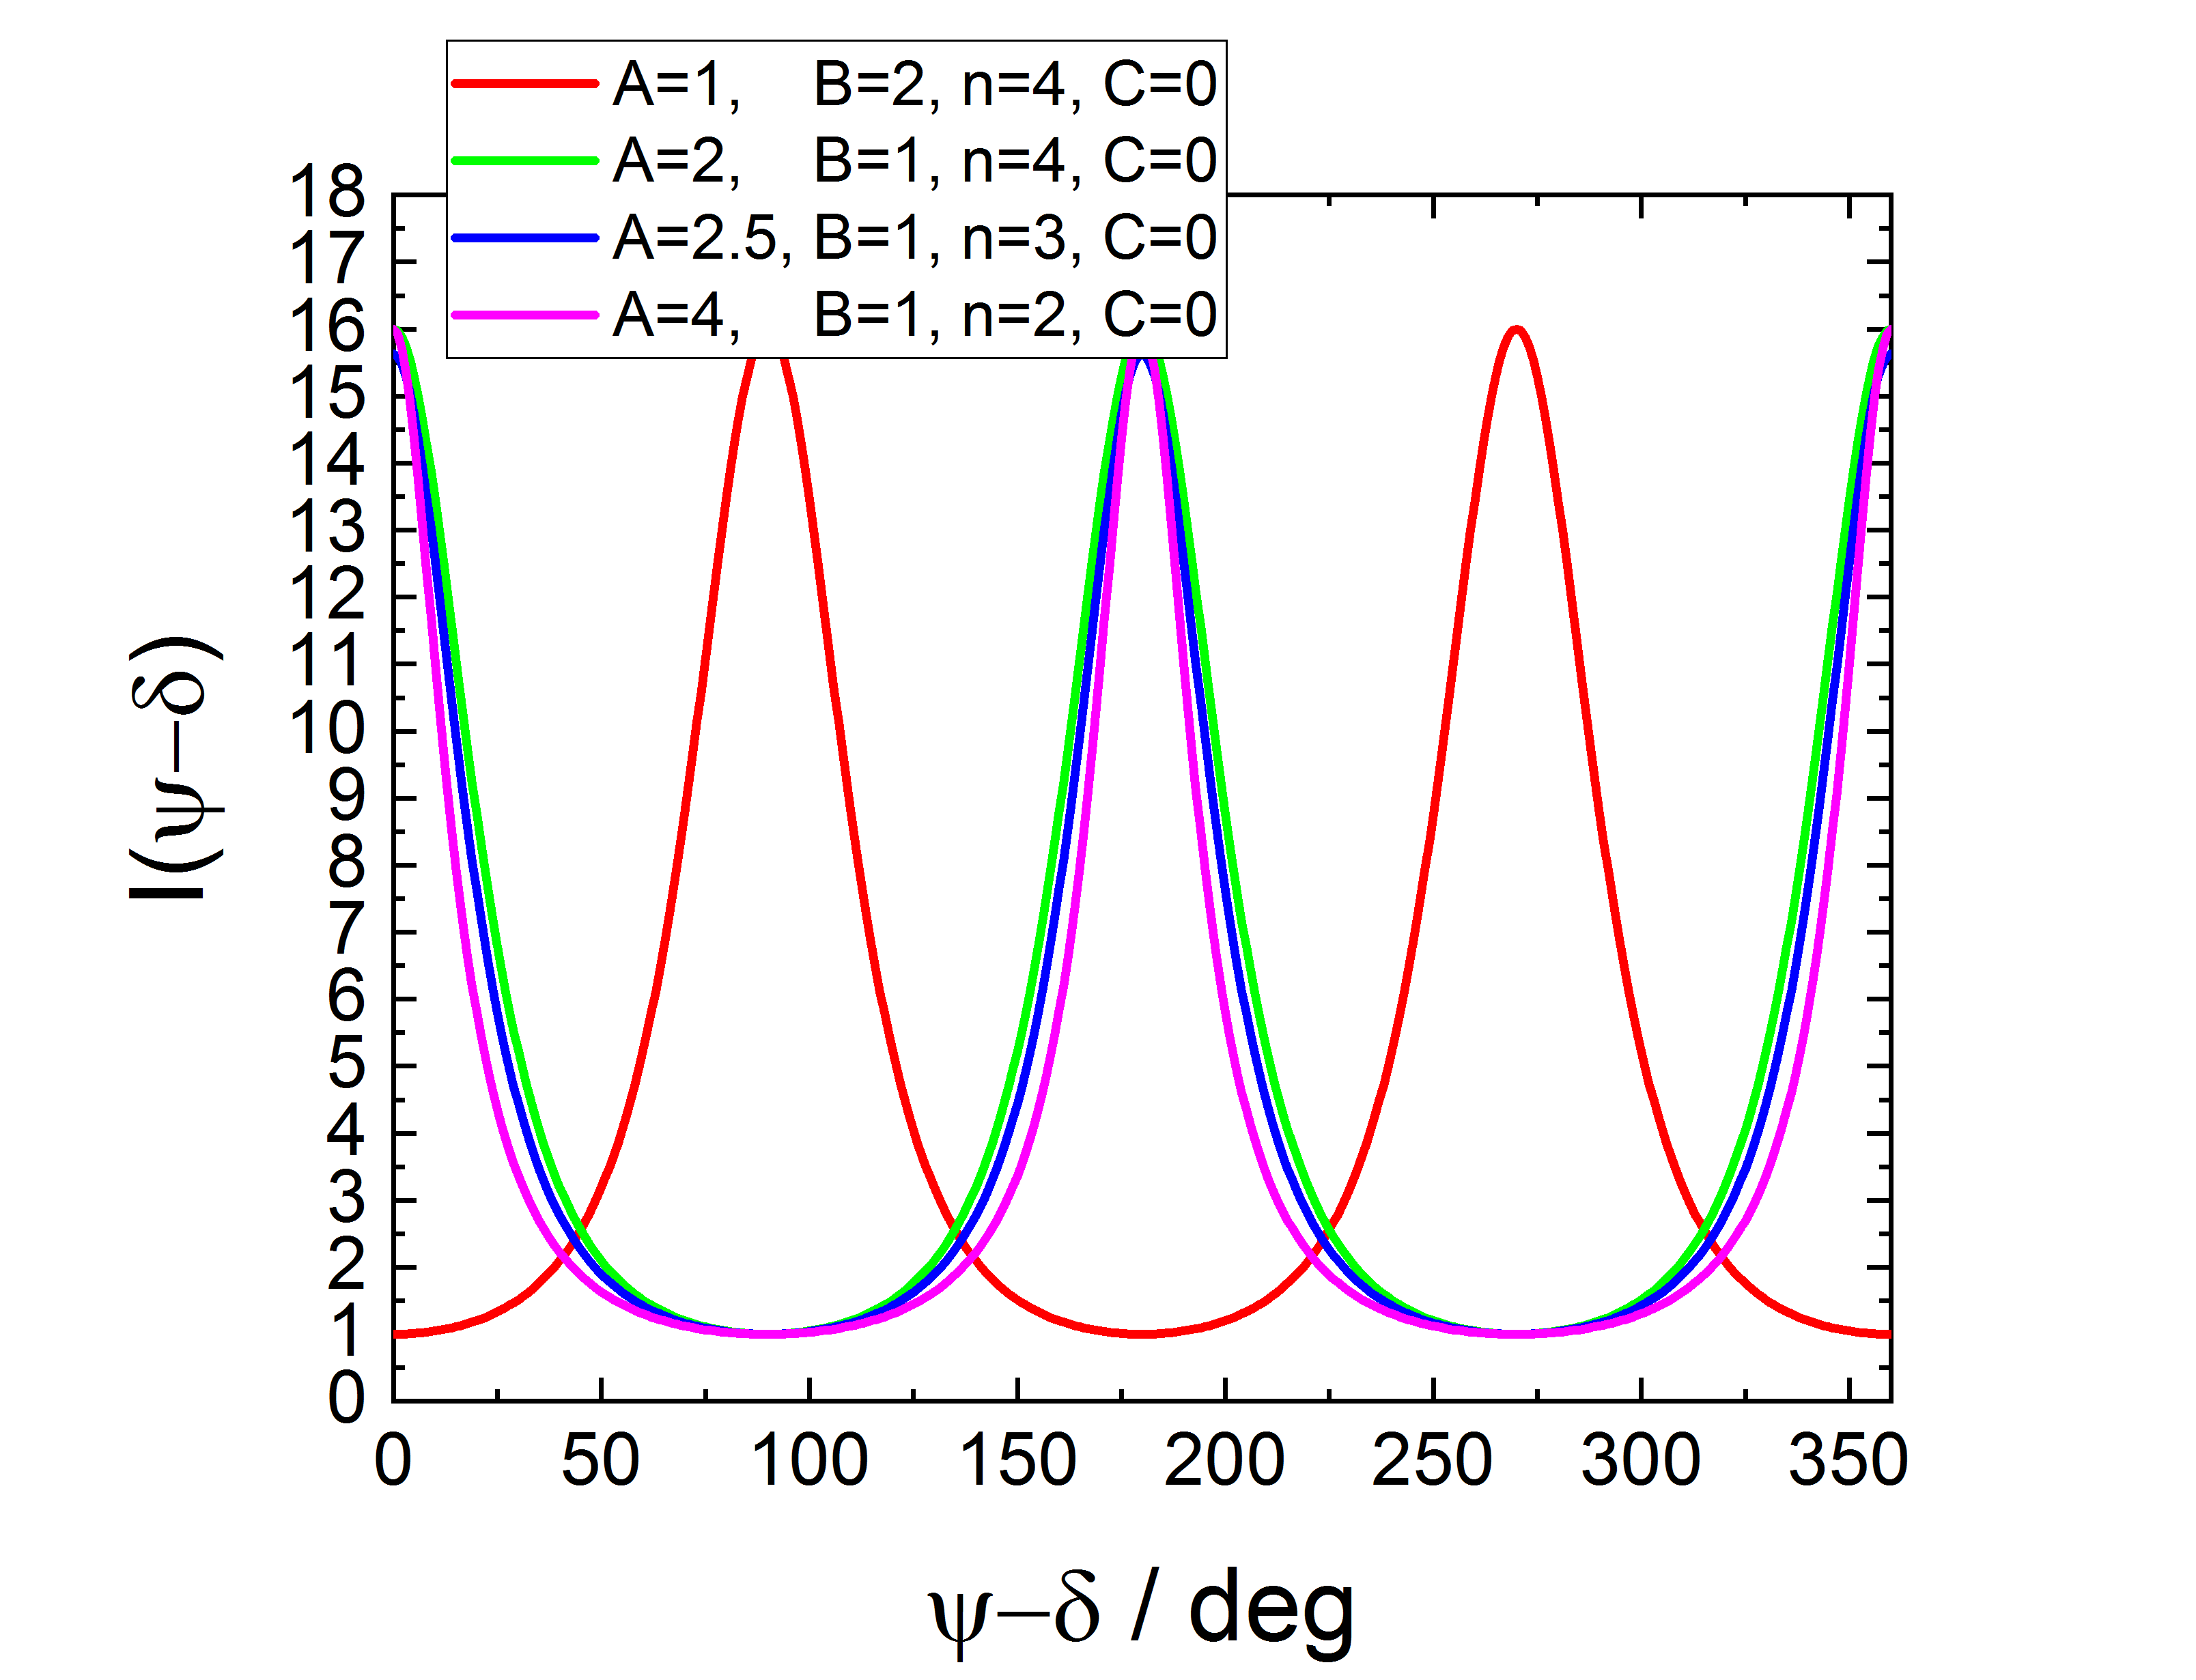
\includegraphics[width=0.7\textwidth]{../images/form_factor/azimuthal/ellipsoidal.png}
\end{center}
\caption{Azimuthal intensity distribution of the elliptically averaged model}
\label{fig:elliptically_averaged}
\end{figure}

\newpage

\subsection{affine shrinkage} ~\\
An affine deformation  profile has been given by \cite{Vilcinskas2015,Zlopasa2015} and reads as
\begin{align}
\mathcal{I}_\mathrm{as}(\psi) &= \lambda^2\frac{\cos^2\left[\arctan\left(\lambda \tan \chi\right)\right]}{\cos^3(\chi)} \\
\chi &= \psi-\delta
\end{align}
where $\lambda$ is the degree of compression. The final model function is than normalized on the average intensity so that the azimuthal intensity distribution is given by
\begin{align}
  I_\mathrm{as}(\chi) &= I_0 + A \frac{\pi}{2}\frac{\mathcal{I}_\mathrm{as}(\chi)}{\int_0^{\pi/2}\mathcal{I}_\mathrm{as}(\chi)\mathrm{d}\chi}
\end{align}

\hspace{1pt}\\
\underline{Input Parameters for models \texttt{affine shrinkage (deg)} and \texttt{affine shrinkage (rad)}:}\\
\begin{description}
\item[\texttt{I0}] flat background $I_0$
\item[\texttt{A}] Amplitude $A$ of the angle dependent intensity
\item[\texttt{lambda}] shrinkage factor $\lambda$
\item[\texttt{delta}] offset of shrinkage direction $\delta$ in degree or radian
\end{description}

\noindent \underline{Note:}
$\lambda$ needs to be a positive nonzero number. $\lambda=1$: no shrinkage, $\lambda>1$: shrinkage, $0<\lambda<1$: swelling.


\begin{figure}[htb]
\begin{center}
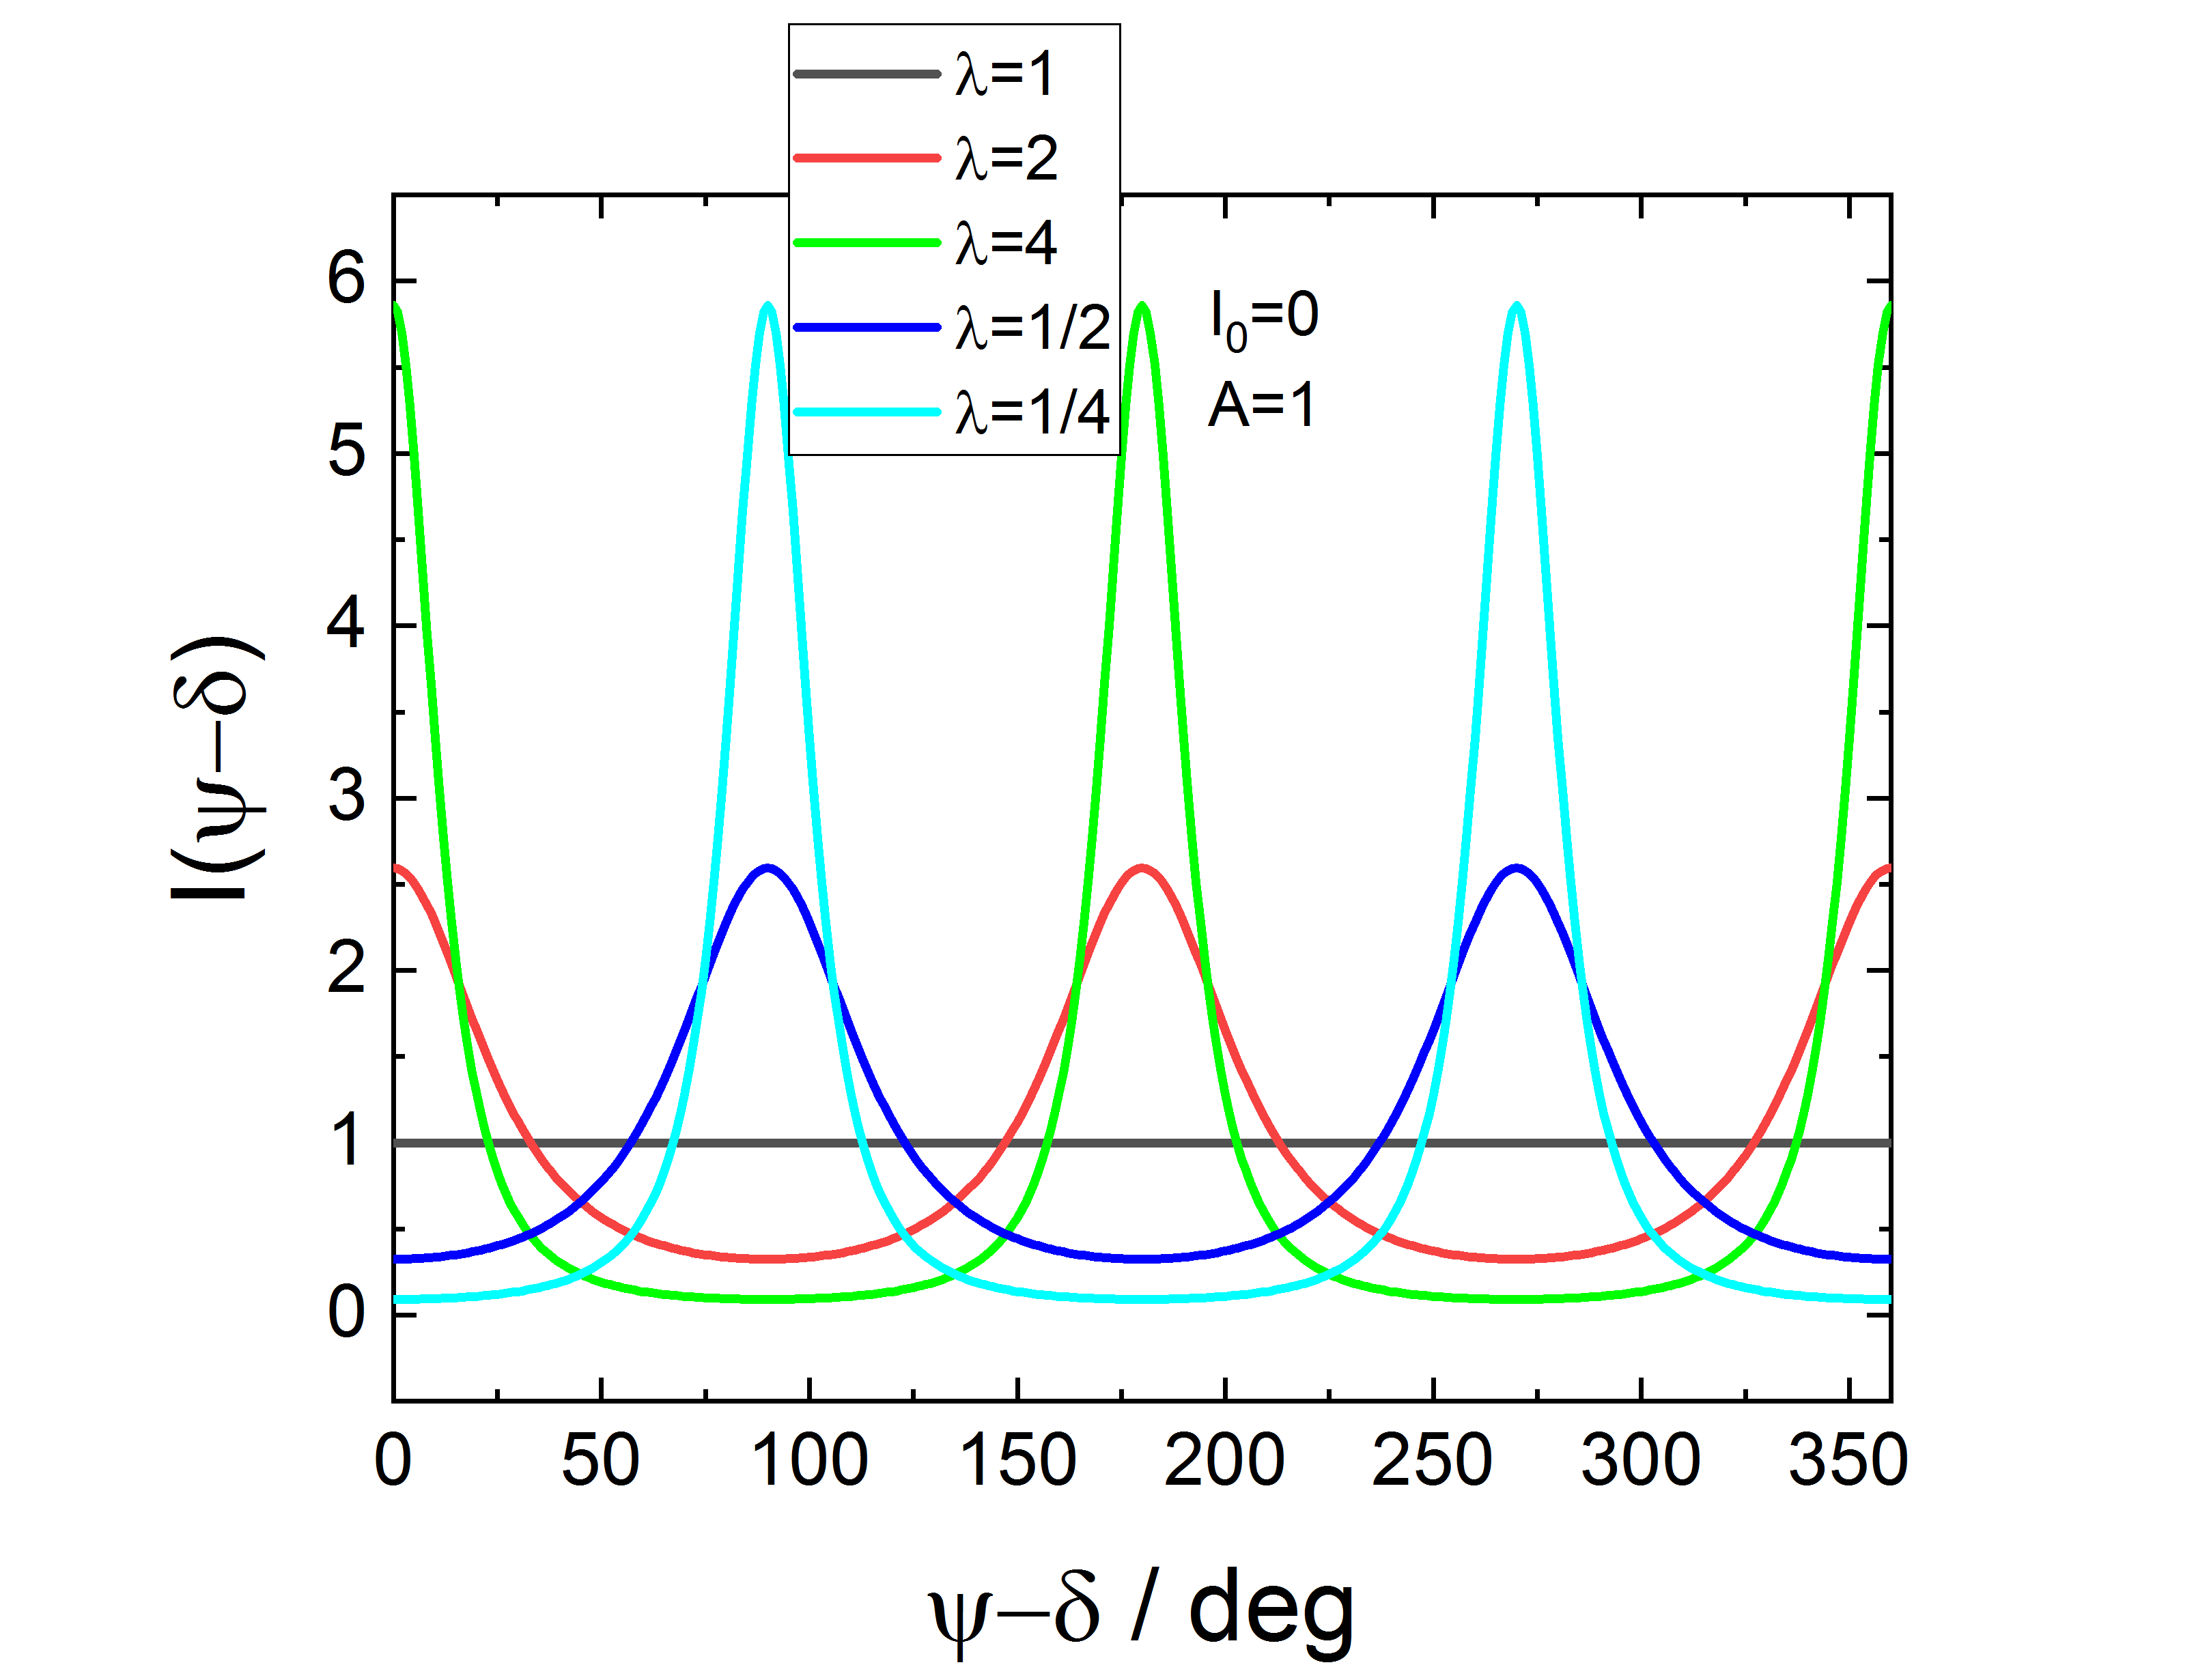
\includegraphics[width=0.7\textwidth]{../images/form_factor/azimuthal/affine_shrinkage.png}
\end{center}
\caption{Azimuthal intensity distribution of the affine shrinkage model}
\label{fig:affineshrinkage}
\end{figure}

\newpage
\subsection{Maier-Saupe azimuthal analysis} ~\\
\label{sec:Picken}

In the Picken model \cite{Picken1990,Fan1994,Makarova2013} the azimuthal intensity reads as
\begin{align}
  \mathcal{I}_\mathrm{P}(\chi) &= \exp\left(\kappa\cos^2\chi\right)\\
\chi &= \psi-\delta
\end{align}
The final model function is than normalized on the average intensity so that the azimuthal intensity distribution is given by
\begin{align}
  I_\mathrm{P}(\chi) &= I_0 + A \frac{\pi}{2}\frac{\mathcal{I}_\mathrm{P}(\chi)}{\int_0^{\pi/2}\mathcal{I}_\mathrm{P}(\chi)\mathrm{d}\chi}
\end{align}

\hspace{1pt}\\
\underline{Input Parameters for models \texttt{MaierSaupe (deg)} and \texttt{MaierSaupe (rad)}:}\\
\begin{description}
\item[\texttt{I0}] flat background $I_0$
\item[\texttt{A}] Amplitude $A$ of the angle dependent intensity
\item[\texttt{kappa}] parameter for strength of orientation $\kappa$
\item[\texttt{delta}] offset $\delta$ in degree or radian
\end{description}

\noindent \underline{Note:}
For $\kappa=0$ the azimuthal intensity is flat, for $\kappa>0$ the highest intensity is in the direction $\psi-\delta=0$ and for $\kappa<0$ in the direction $\psi-\delta=\pi/2$

\begin{figure}[htb]
\begin{center}
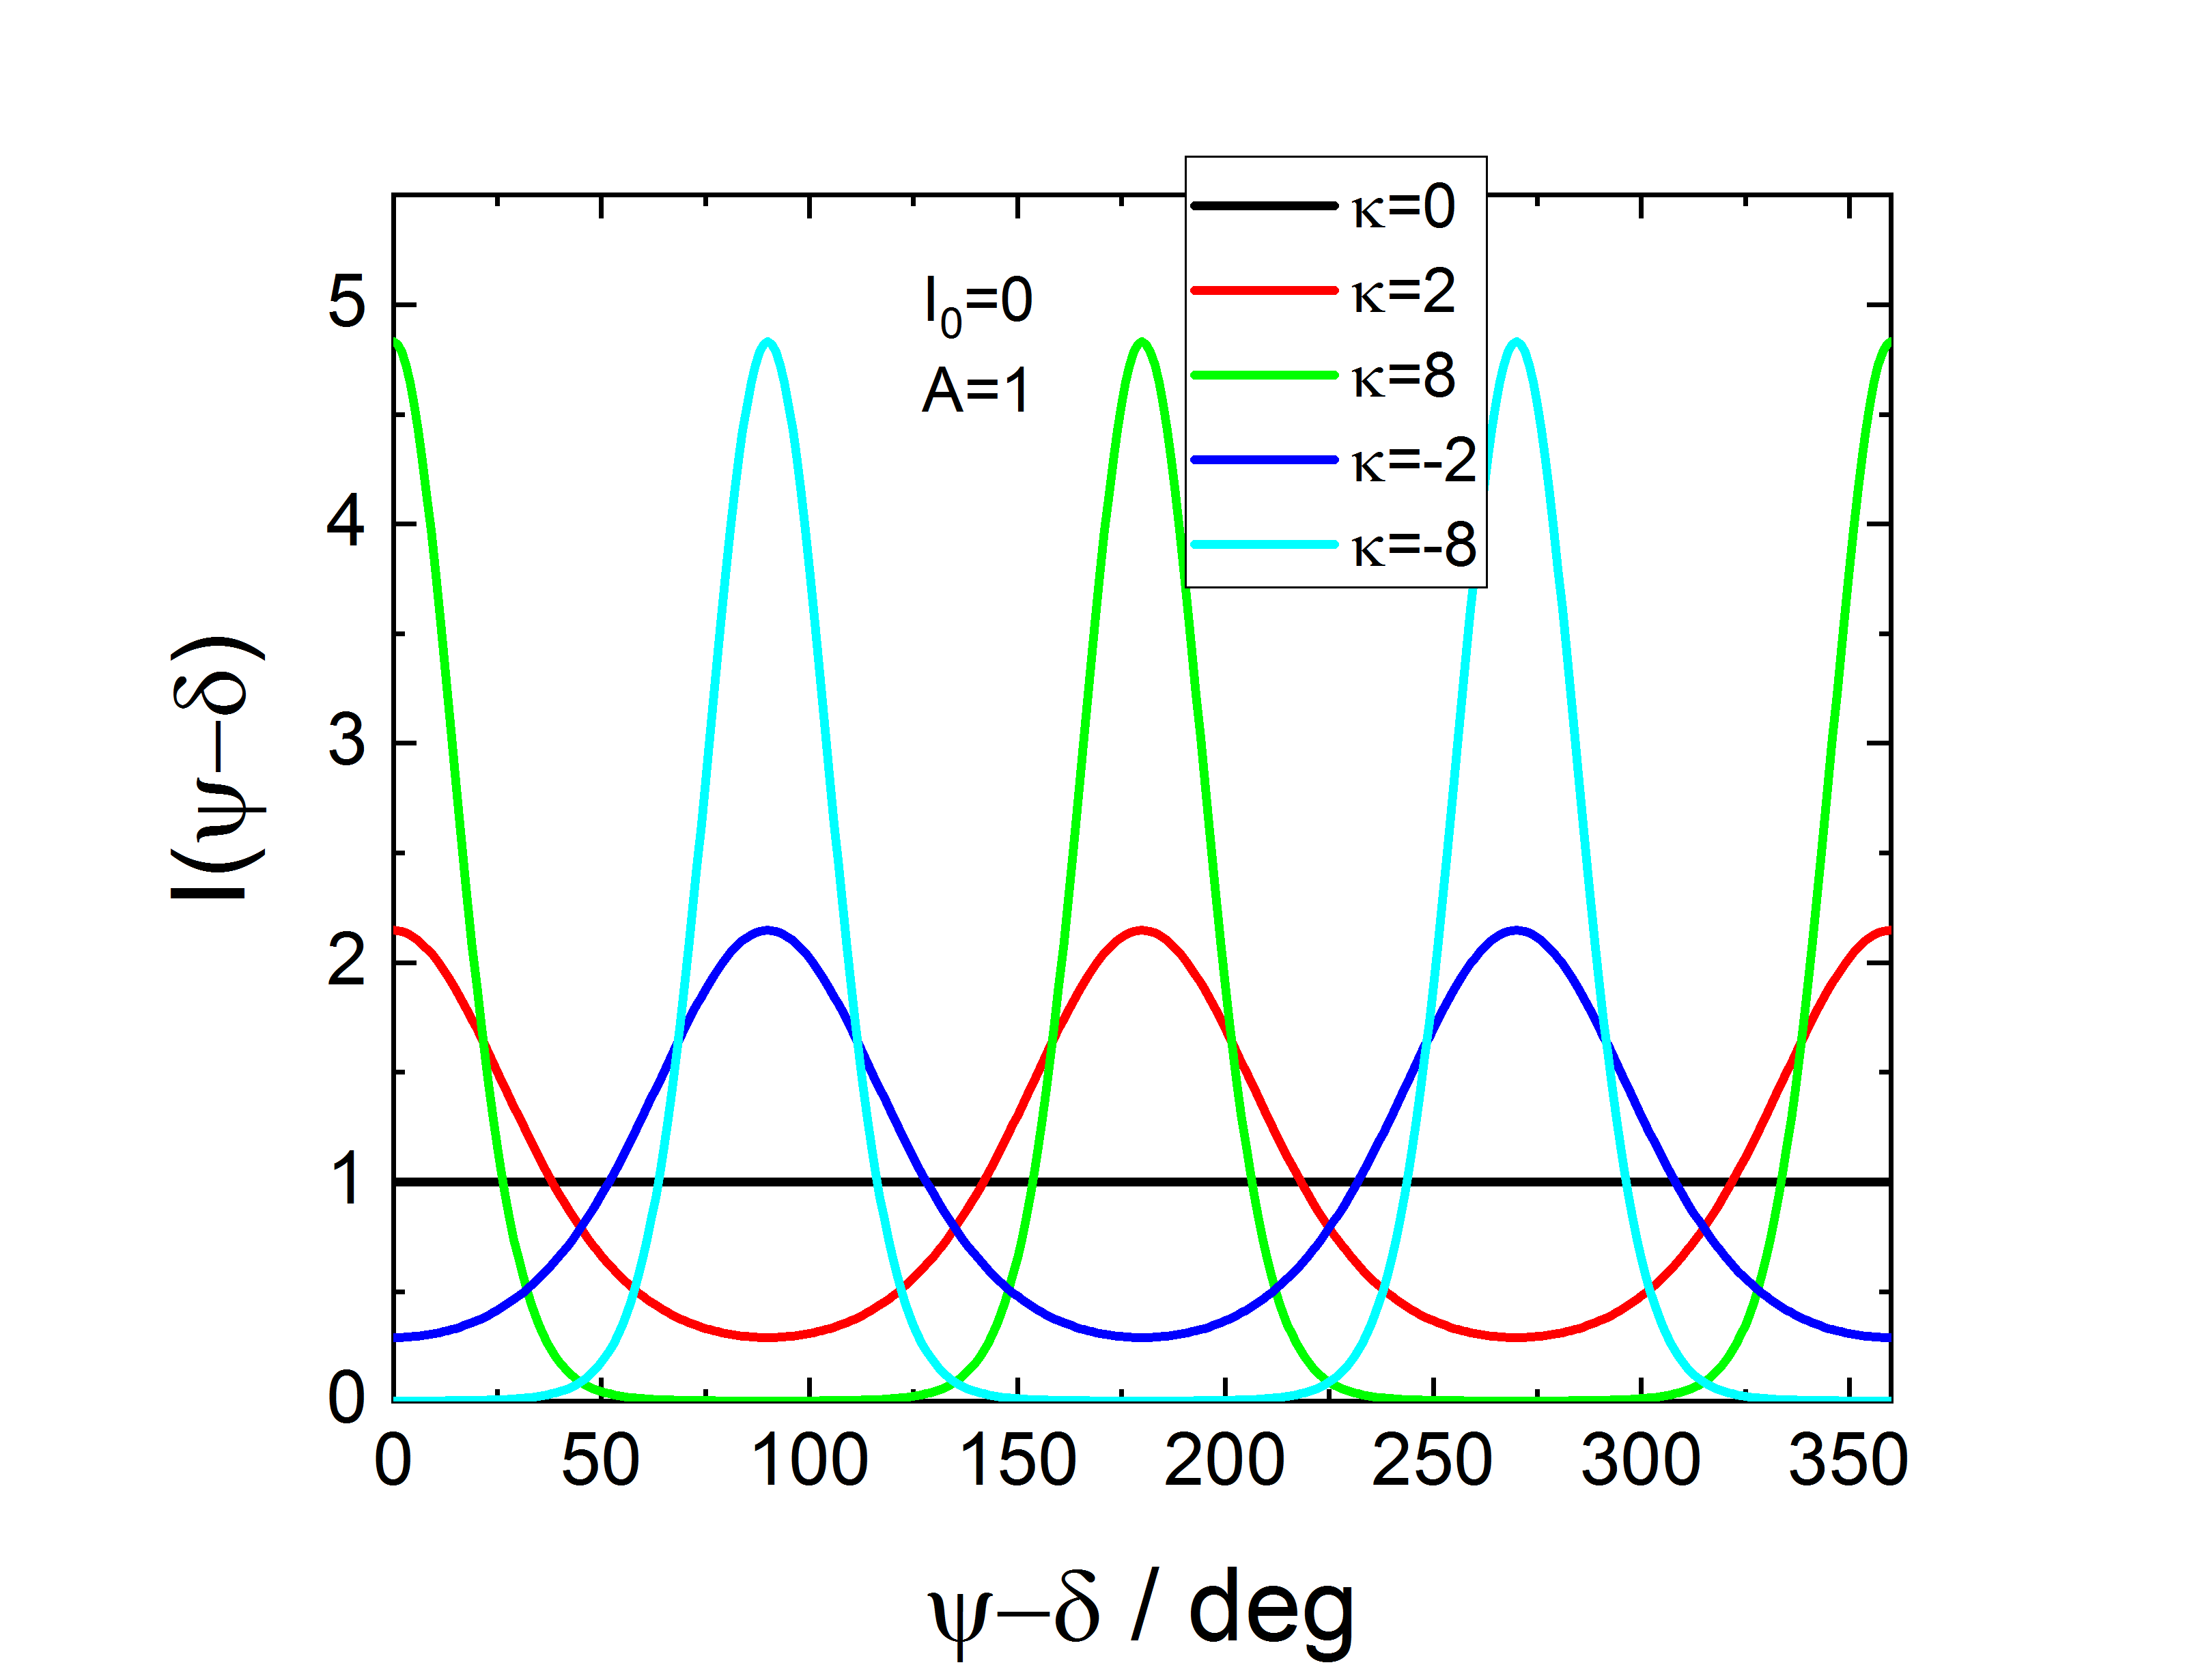
\includegraphics[width=0.7\textwidth]{../images/form_factor/azimuthal/maiersaupe.png}
\end{center}
\caption{Azimuthal intensity distribution of the Maier-Saupe model from Picken \cite{Picken1990}}
\label{fig:maiersaupe}
\end{figure}

\newpage
\subsection{azimuthal analysis of very long oriented structures with Maier-Saupe or Onsager orientation distribution} ~\\
\label{sec:azimuthalVeryLongStructures}
X-ray scattering has been used to obtain order parameters of liquid crystals. A work of Leadbetter and Norris \cite{Leadbetter1979} describe the underlying assumptions and derived the equation
\begin{align}
\mathcal{I}_\mathrm{LN}(\chi) &= \int_{\theta=\chi}^{\pi/2} \frac{p(\theta) \sin\theta}{\cos^2\chi \sqrt{\tan^2\theta-\tan^2\chi}} \mathrm{d}\theta
\end{align}
where $p(\theta) \sin\theta$ describe the orientation distribution of the molecular axis towards the preferred direction $\theta$. Later on it was recognized by Burger and Ruland \cite{Burger2006} that the formula contains an error and has to be corrected according to an equation derived earlier by Kratky \cite{Kratky1933}. The correct equation  which was also re-derived by Mills \cite{Mills2008} reads as \cite{Sims2018,Agra-Kooijman2017}
\begin{align}
\mathcal{I}_\mathrm{K}(\chi) &= \int_{\theta=\chi}^{\pi/2} \frac{p(\theta) \sin\theta}{\sqrt{\cos^2\chi-\cos^2\theta}} \mathrm{d}\theta = \int_{\theta=\chi}^{\pi/2} \frac{p(\theta) \sin\theta}{\sqrt{\sin^2\theta-\sin^2\chi}} \mathrm{d}\theta\\
&= \int_{\theta=\chi}^{\pi/2} \frac{p(\theta) \tan\theta}{\cos\chi \sqrt{\tan^2\theta-\tan^2\chi}} \mathrm{d}\theta
\end{align}
with $\chi = \psi-\delta$.  The final model function is than normalized on the average intensity so that the azimuthal intensity distribution is given by
\begin{align}
  I_\mathrm{LN}(\chi) &= I_0 + A \frac{\pi}{2}\frac{\mathcal{I}_\mathrm{LN}(\chi)}{\int_0^{\pi/2}\mathcal{I}_\mathrm{LN}(\chi)\mathrm{d}\chi} \\
  I_\mathrm{K}(\chi) &= I_0 + A \frac{\pi}{2}\frac{\mathcal{I}_\mathrm{K}(\chi)}{\int_0^{\pi/2}\mathcal{I}_\mathrm{K}(\chi)\mathrm{d}\chi}
\end{align}
For the two approximations, the in principle obsolete Leadbetter and Norris one and the correct Kratky approximation, the Maier-Saupe and the Onsager orientation distribution have been implemented.

\hspace{1pt}\\
\underline{Input Parameters for models} \\
\underline{\texttt{azimuthal (long cyl.,MS,K,deg)}}, \underline{\texttt{azimuthal (long cyl.,MS,K,rad)}}, \underline{\texttt{azimuthal (long cyl.,Onsager,K,deg)}}, \underline{\texttt{azimuthal (long cyl.,Onsager,K,rad)}}, \underline{\texttt{azimuthal (long cyl.,MS,LN,deg)}}, \underline{\texttt{azimuthal (long cyl.,MS,LN,rad)}}, \underline{\texttt{azimuthal (long cyl.,Onsager,LN,deg)}}, \underline{\texttt{azimuthal (long cyl.,Onsager,LN,rad)}:}\\
\begin{description}
\item[\texttt{I0}] flat background $I_0$
\item[\texttt{A}] Amplitude $A$ of the angle dependent intensity
\item[\texttt{kappa}] width $\kappa$ of orientation distribution
\item[\texttt{delta}] direction offset $\delta$ in degree or radian
\end{description}

\newpage
\noindent \underline{Note:}
\begin{itemize}
  \item The integrals for $\mathcal{I}_\mathrm{K}(\chi)$ and $\mathcal{I}_\mathrm{LN}(\chi)$ around $\chi\simeq\pi/2$ become numerical unstable and are fixed to the value at $(1-10^{-4})\pi/2$.
  \item For the Maier-Saupe orientation distribution in the Kratky approximation the analytical solution given by \cite{Mills2008} has been implemented.
\end{itemize}

\begin{figure}[htb]
\begin{center}
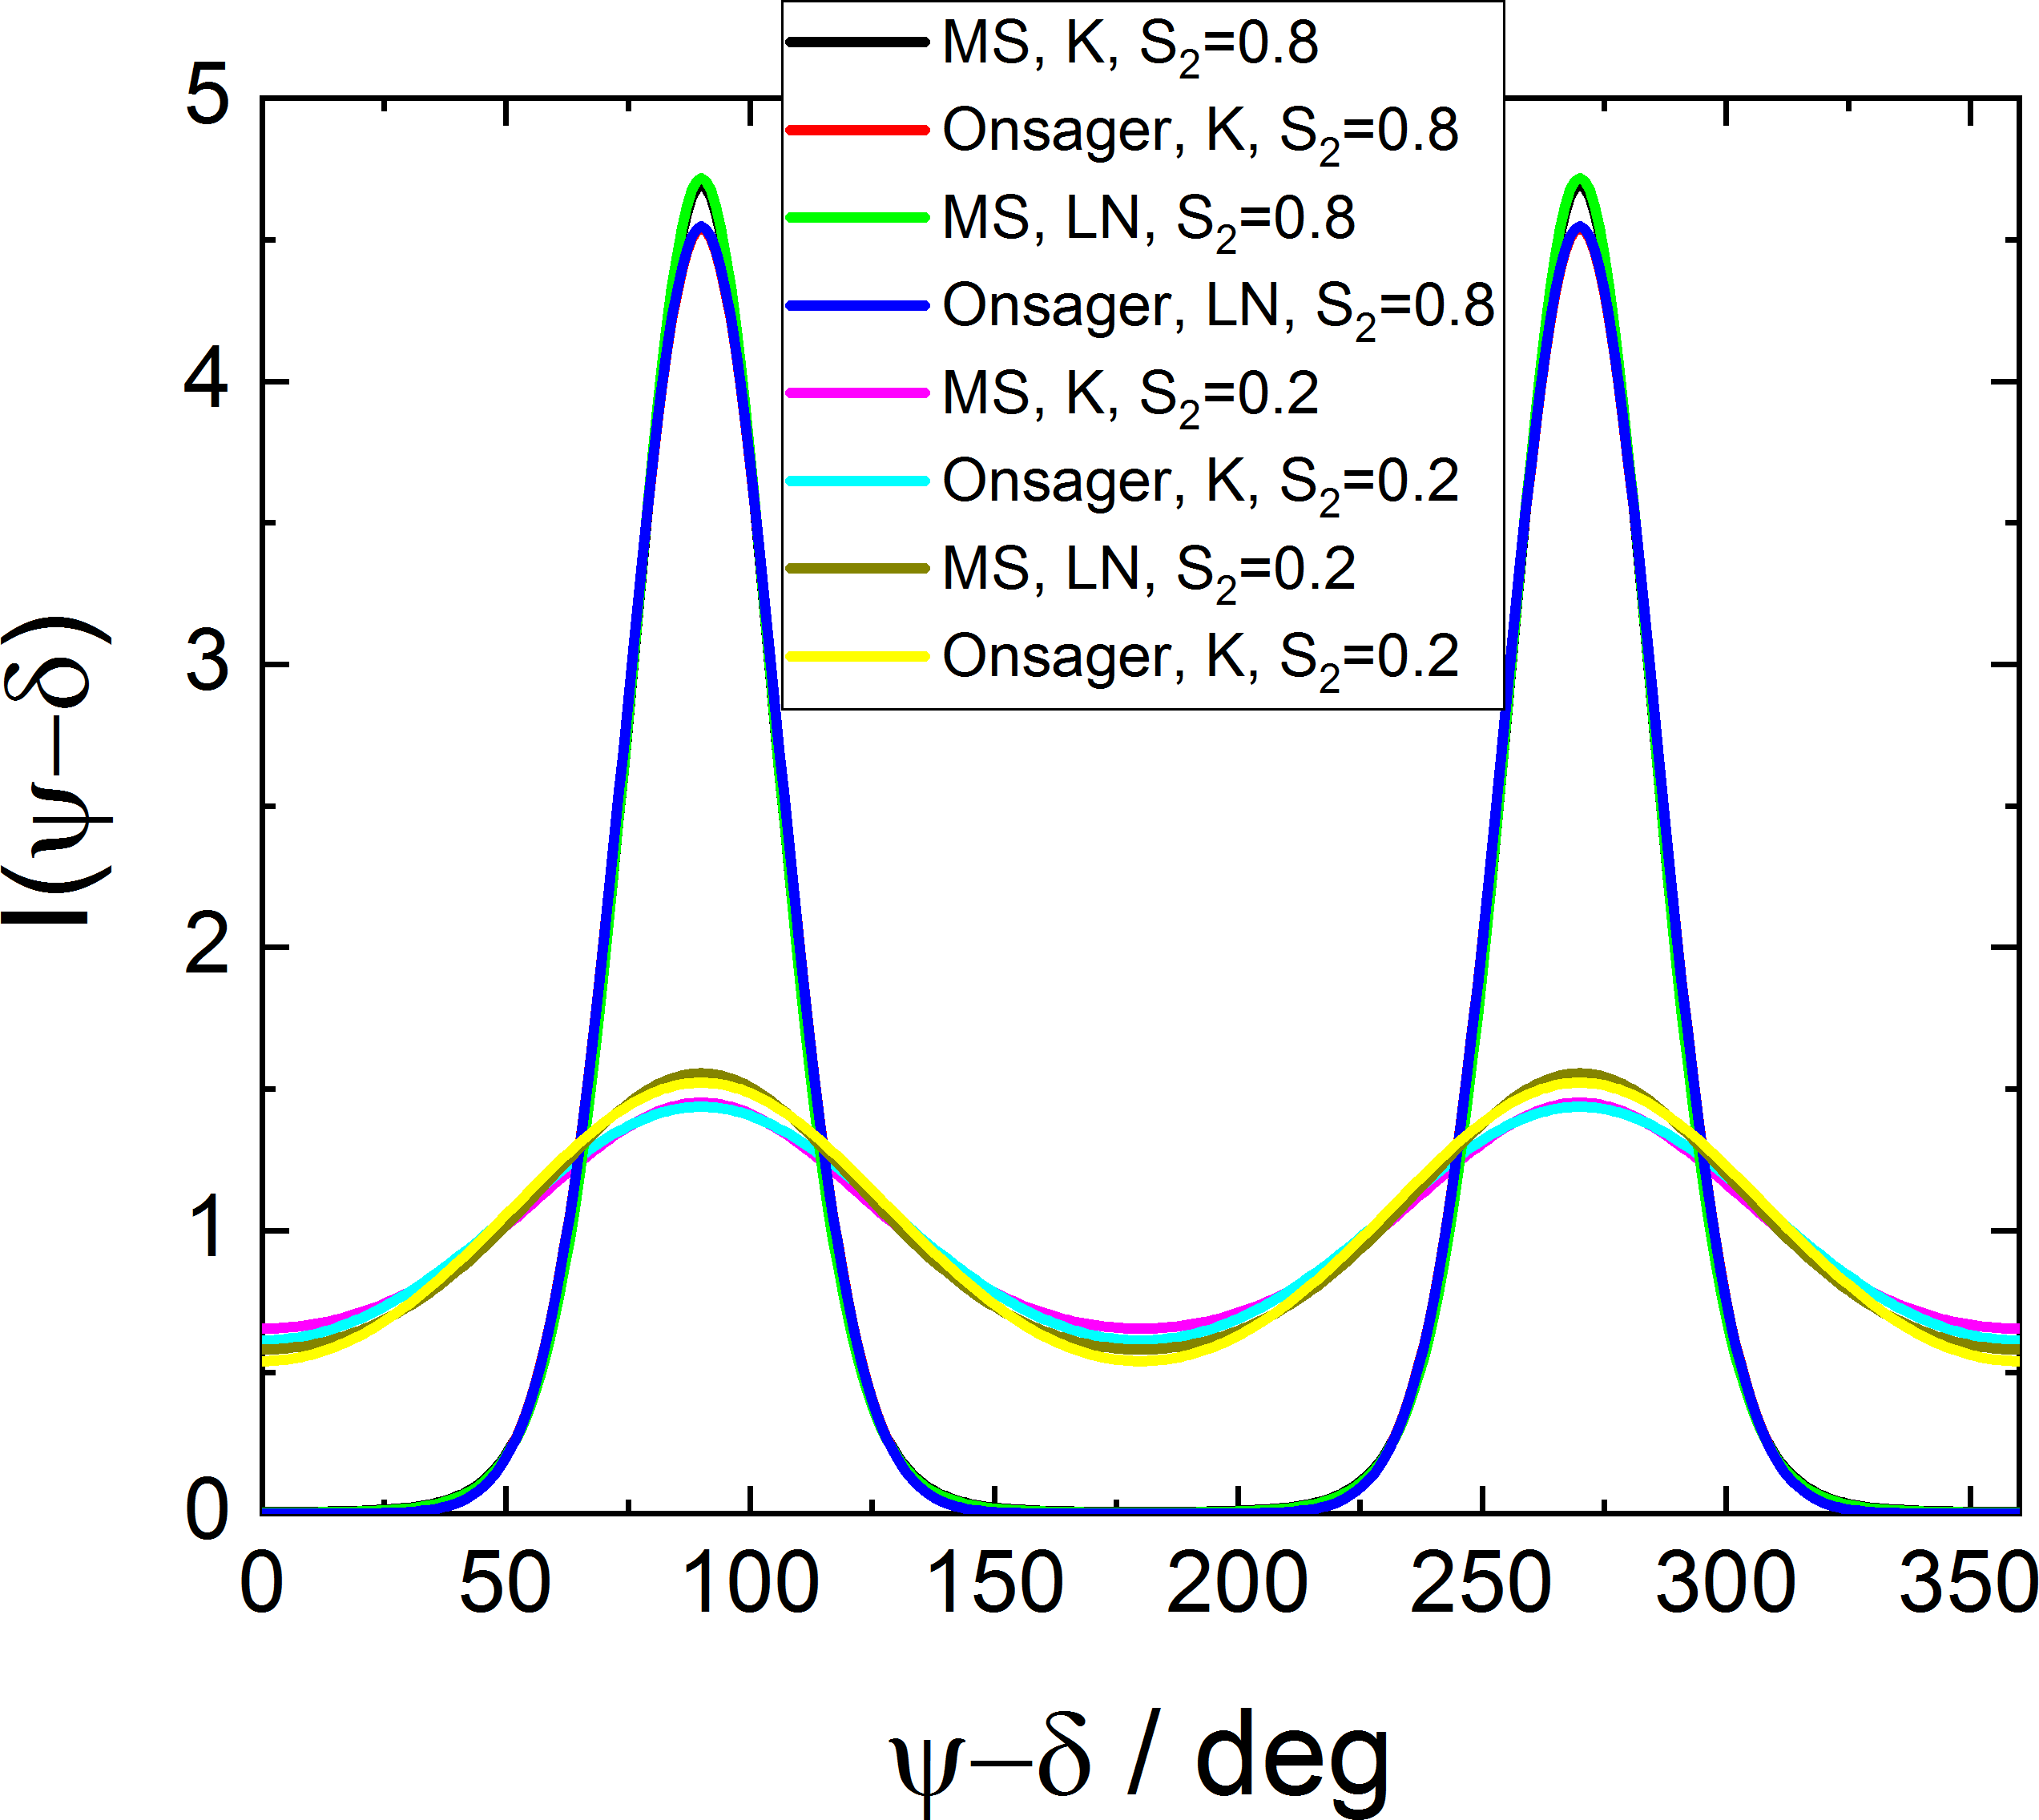
\includegraphics[width=0.7\textwidth]{../images/form_factor/azimuthal/azimuthal_long_cylinder.png}
\end{center}
\caption{Azimuthal intensity distribution according to the correct Kratky approximation and the obsolete Leadbetter with a Maier-Saupe and Onsager orientation distribution. The parameters of the orientation distributions have been chosen so that their order parameter is $S_2=0.8$ and $S_2=0.2$.}
\label{fig:azimuthal_long_cylinder}
\end{figure}

\newpage
\subsection{azimuthal analysis of sheared or deformed structures} ~\\
A couple of models of sheared and deformed form factors are described in section \ref{sec:ShearedAndDeformed}. All these form factors have an parameter $\psi$ describing the direction of the scattering vector towards the symmetry axis of the textured sample (e.g.\ due to shear of deformation). Some of these functions have been supplied so that they become a function of $\psi$ instead of $q$, to be able to describe not sector averaged data $I(q;\psi,\ldots)$ but rather azimuthal data at a fixed scattering vector $I(\psi;q,\ldots)$. The form factor from section \ref{sect:ShearedCylinderHayterPenfold} and \ref{sect:partlyalignedCylShell} have been made available. If the azimuthal plot is supplied by an appropriate $q$-value it is often an advantage not to use the full model description but rather the approximations given by the models in the previous sections \ref{sec:Picken} and \ref{sec:azimuthalVeryLongStructures}.

\begin{figure}[htb]
\captionsetup[subfigure]{position=b}
\centering
\subcaptionbox{Scattering curve $I(q)$ of a long cylinder aligned according to a Maier-Saupe orientation distribution \label{fig:comparisionOfAzimuthalIntModels1} }{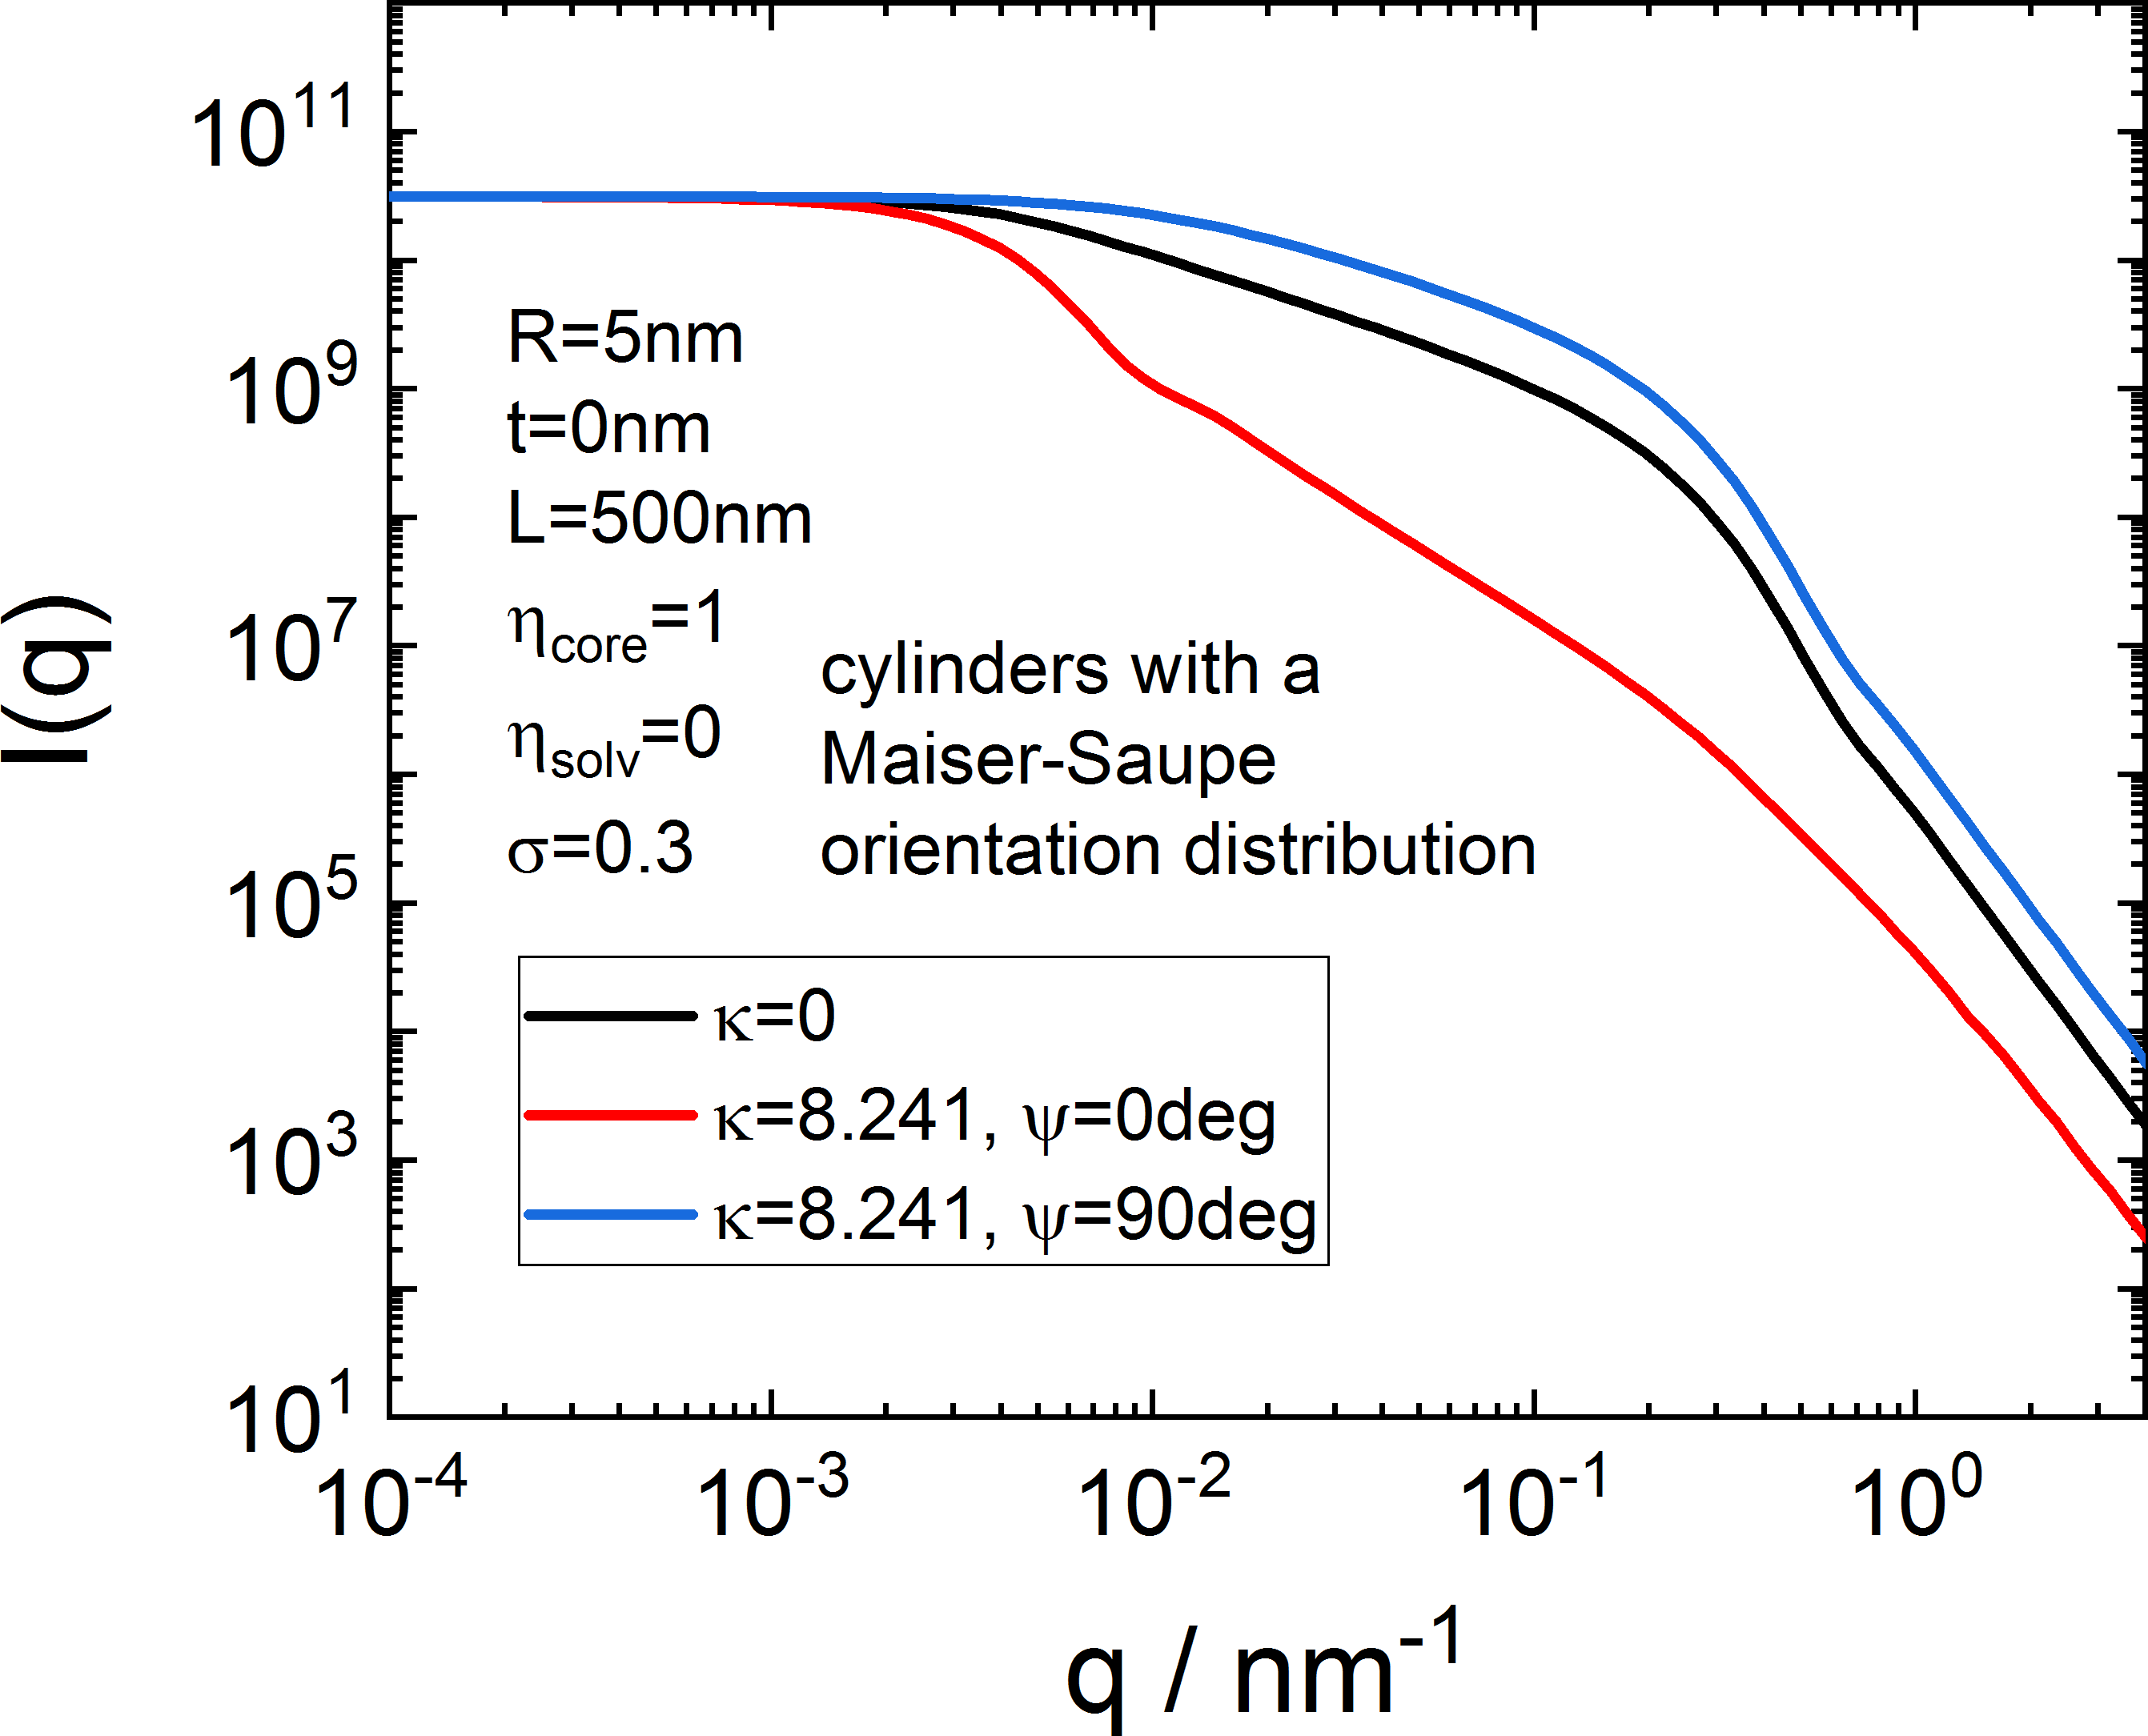
\includegraphics[width=0.48\textwidth]{../images/form_factor/azimuthal/I(Q)_MS_Cylinder.png}}
\hfill
\subcaptionbox{Azimuthal intensity distribution $I(\psi)$ of the same model as on the left \label{fig:comparisionOfAzimuthalIntModels2} }{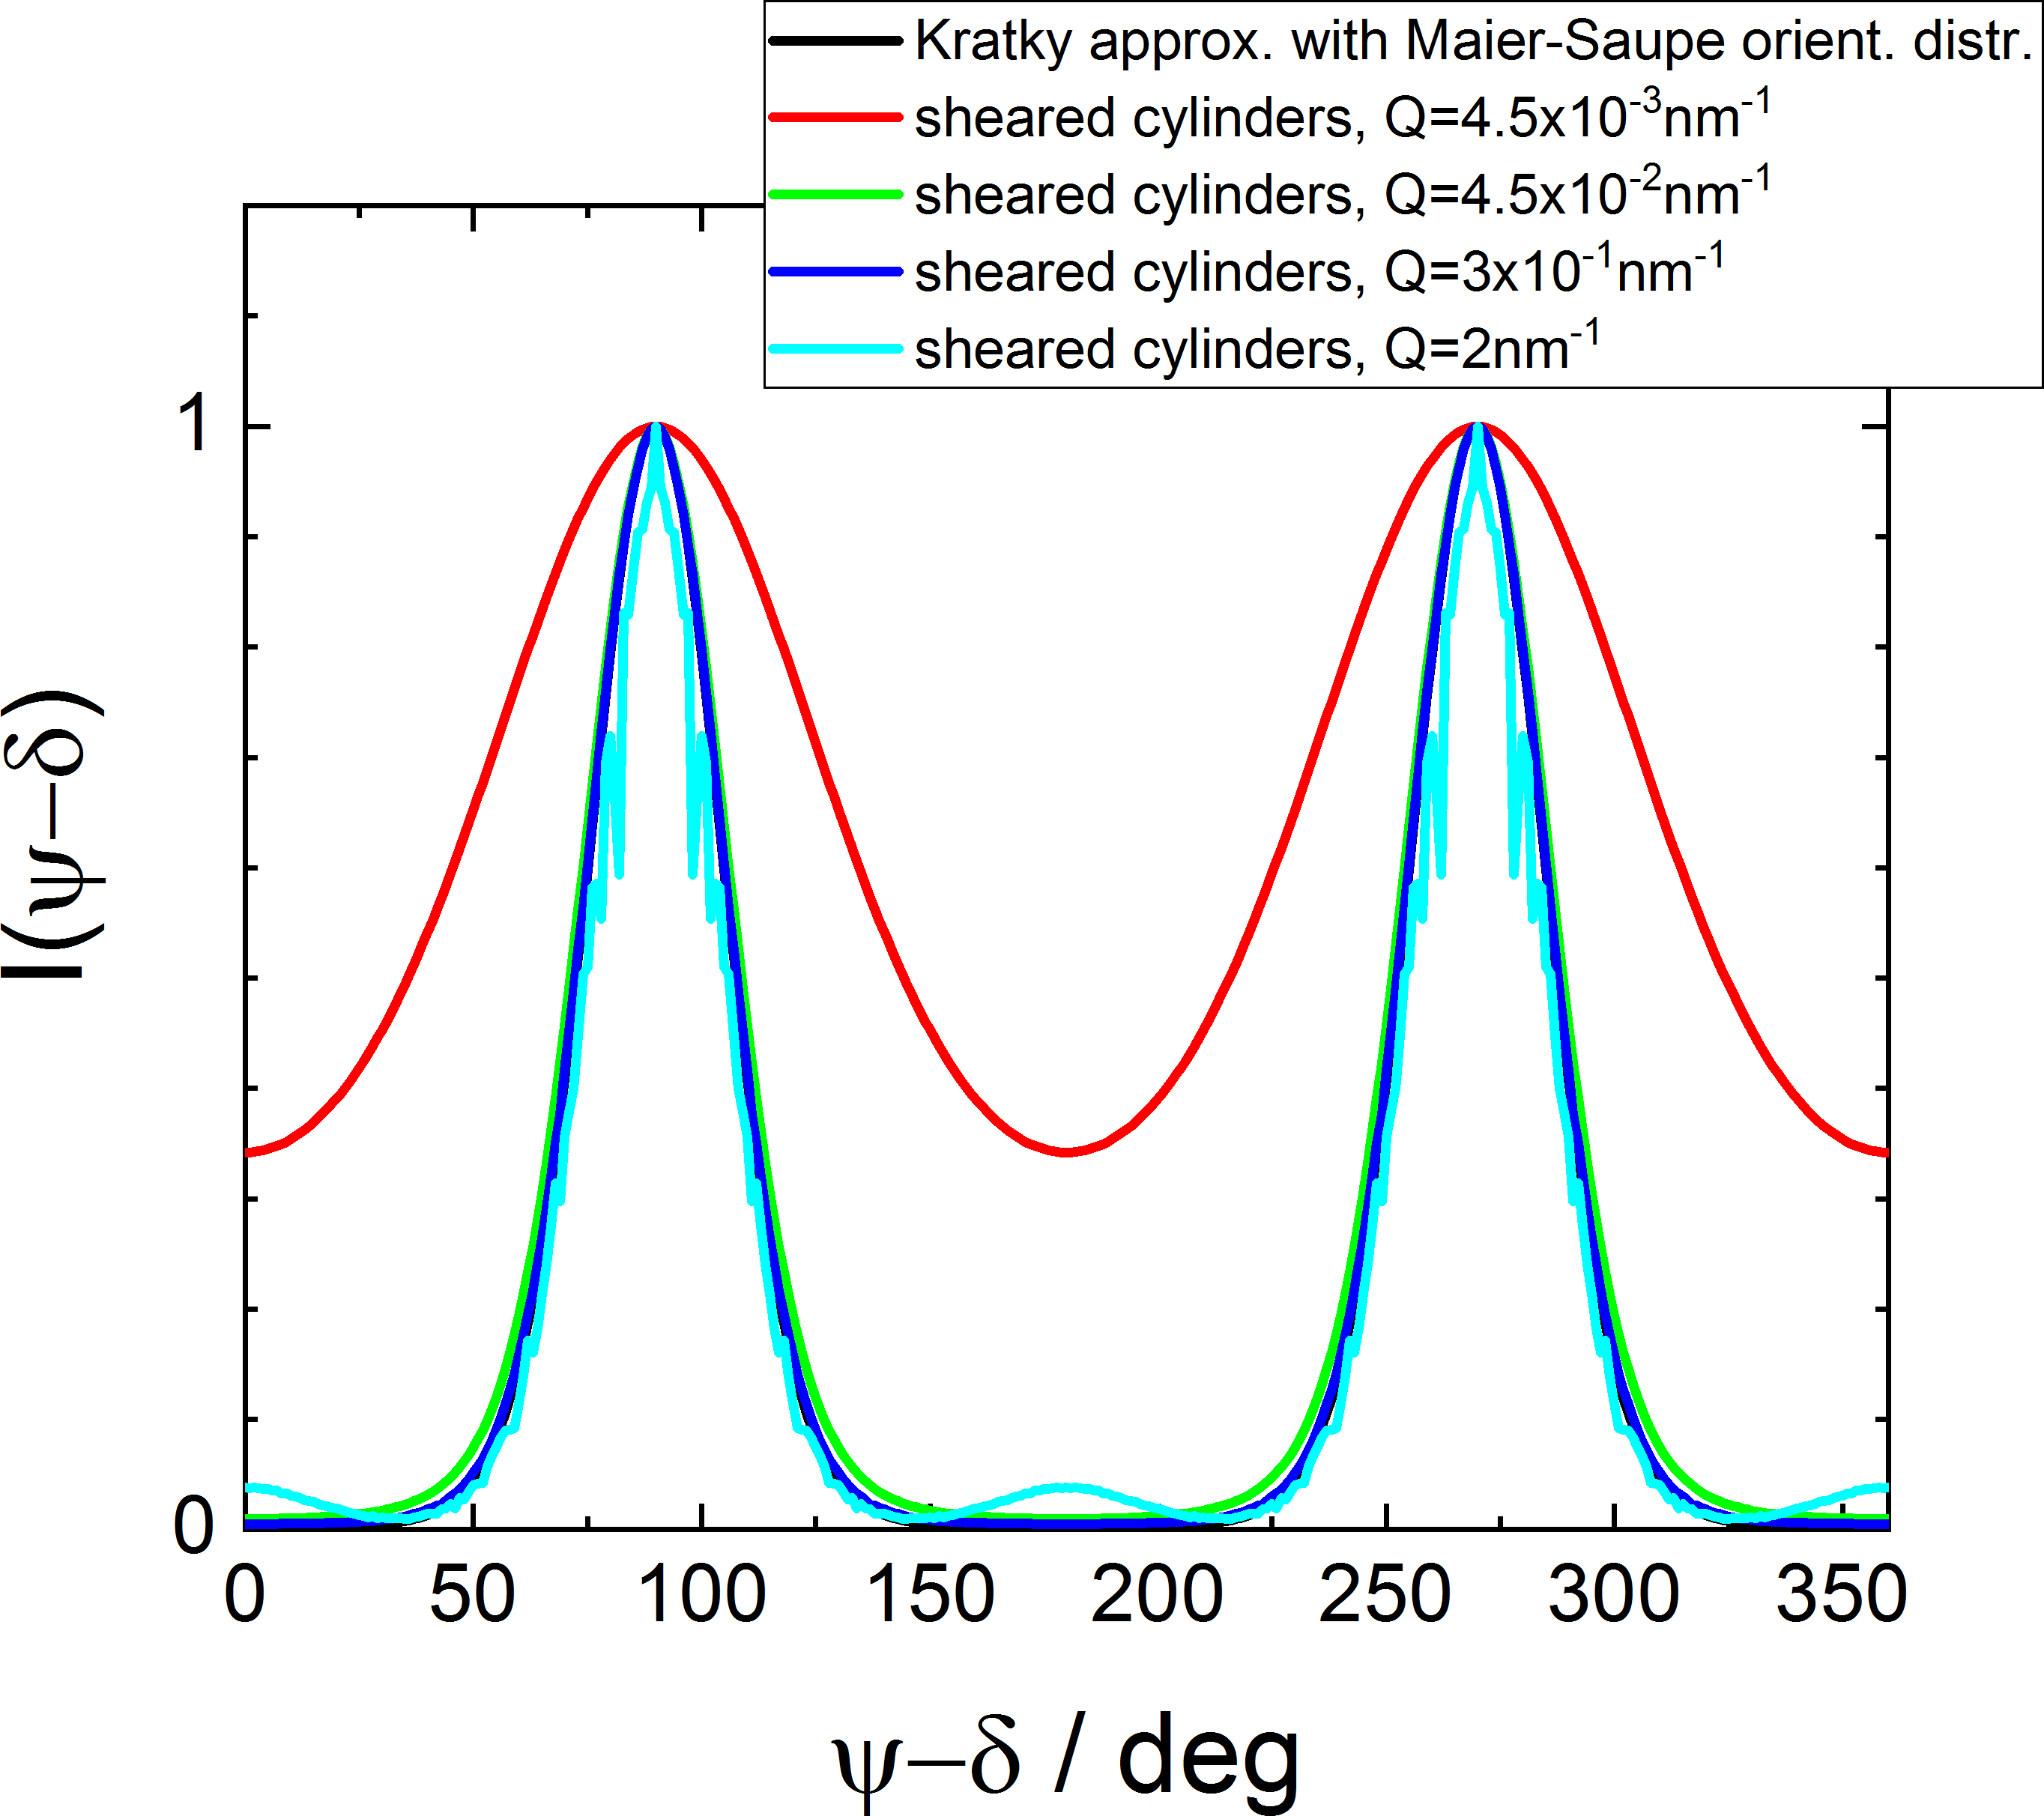
\includegraphics[width=0.48\textwidth]{../images/form_factor/azimuthal/I(PSI)_MS_Cylinder.png}}
\caption{The approximations made by Kratky, Leadbetter and Pickens in the previous sections seems to hold in the intermediate $q$-range, but not in the Porod-regime or Guinier-regime of the cylinders}
\label{fig:comparisionOfAzimuthalIntModels}
\end{figure}

\hspace{1pt}\\
The input parameters are the same as those in \ref{sect:ShearedCylinderHayterPenfold} and \ref{sect:partlyalignedCylShell}, except that $q$ and $\psi$ have been exchanged.\\
\underline{Input Parameters for model}\\ \underline{\texttt{Sheared Cylinders (Maier-Saupe) azimuthal}}, \underline{\texttt{Sheared Cylinders (Gauss) azimuthal}}, \underline{\texttt{Sheared Cylinders (Boltzmann) azimuthal}}, \underline{\texttt{Sheared Cylinders (Onsager) azimuthal}}, \underline{\texttt{Sheared Cylinders (Heavyside) azimuthal}}, \underline{\texttt{Sheared Cylinders (Hayter-Penfold) azimuthal}}:\\
\begin{description}
\item[\texttt{R}] radius of cylinders $R$
\item[\texttt{t}] shell thickness $t$
\item[\texttt{L}] cylinder length $L$
\item[\texttt{eta\_core}] scattering length density of cylinder core $\eta_\mathrm{core}$
\item[\texttt{eta\_shell}] scattering length density of cylinder shell $\eta_\mathrm{shell}$
\item[\texttt{eta\_solv}] scattering length density of solvent $\eta_\mathrm{solv}$
\item[\texttt{Q}] scattering vector $Q$
\item[{\texttt{sigma}}] width parameter of lognormal size distribution $\sigma$
\item[{\texttt{kappa}}] orientation distribution parameter $\kappa$
\end{description}

\vspace{5mm}

\underline{Input Parameters for model}\\ \underline{\texttt{Sheared Spheroids (Maier-Saupe) azimuthal}}, \underline{\texttt{Sheared Spheroids (Gauss) azimuthal}}, \underline{\texttt{Sheared Spheroids (Boltzmann) azimuthal}}, \underline{\texttt{Sheared Spheroids (Onsager) azimuthal}}, \underline{\texttt{Sheared Spheroids (Heavyside) azimuthal}}, \underline{\texttt{Sheared Spheroids (Hayter-Penfold) azimuthal}}:\\
\begin{description}
\item[\texttt{R\_equatorial}] equatorial semi-axes of spheroids $R_\mathrm{e}$
\item[\texttt{t}] shell thickness $t$
\item[\texttt{R\_polar}] polar semi-axis of spheroids $R_\mathrm{p}$
\item[\texttt{eta\_core}] scattering length density of cylinder core $\eta_\mathrm{core}$
\item[\texttt{eta\_shell}] scattering length density of cylinder shell $\eta_\mathrm{shell}$
\item[\texttt{eta\_solv}] scattering length density of solvent $\eta_\mathrm{solv}$
\item[\texttt{Q}] scattering vector $Q$
\item[{\texttt{sigma}}] width parameter of lognormal size distribution $\sigma$
\item[{\texttt{kappa}}] orientation distribution parameter $\kappa$
\end{description}

\vspace{5mm}

\noindent \underline{Note:}
\begin{itemize}
\item The size distribution is taken simultaneously over all parameters $R$, $t$, $L$, and $R_\mathrm{e}$, $t$, $R_\mathrm{p}$ respectively, so that their aspect ratios always stay constant.
\item The numerics becomes instable at large $q$-values and t the same time high order parameters.
\end{itemize}
